\chapter{\selectlanguage{greek}Αποτελέσματα}
% Some examples illustrating the dependence on bunch intensity, bunch length and transverse size, plus at least on example from the multi-bunch simulations.


\section{Επίδραση παραμέτρων του επιταχυντή στην ανίχνευση της δέσμης}

\subsection{Αποτελέσματα θεωρητικού μοντέλου}
Τα αποτελέσματα της ανάλυσης που παρουσιάστηκε στην υπο-ενότητα \ref{sub:variable-analysis-MATLAB} φαίνονται παρακάτω.

\begin{figure}[tph]	
	\begin{subfigure}{0.45\textwidth}
		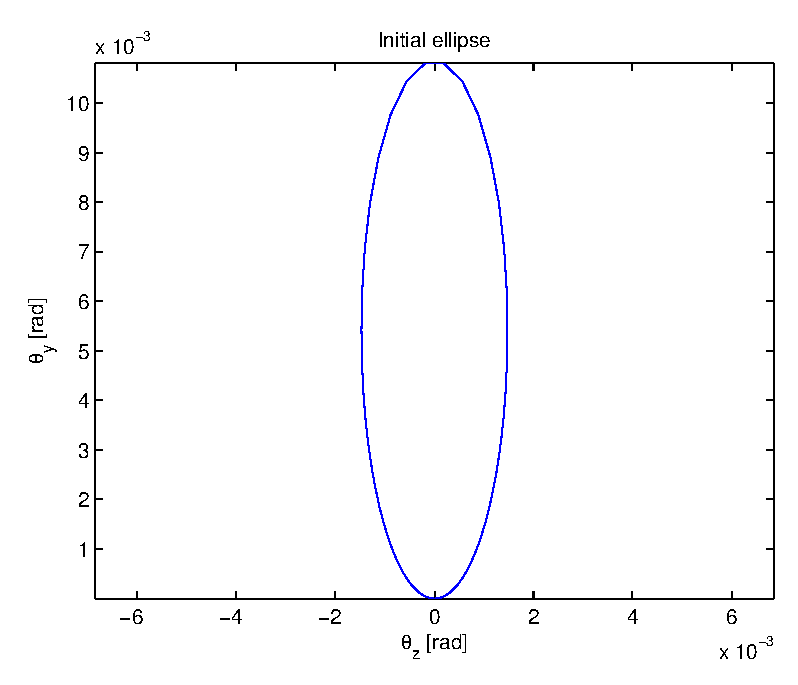
\includegraphics[width=0.9\linewidth]{figures/beam-deflection-script-01-initial-elipse}
		\centering
		\caption{Η χαρακτηριστική έλλειψη στην αρχική κατάσταση}
		\label{fig:beam-deflection-script-01-initial-elipse}
	\end{subfigure}
	~
	\begin{subfigure}{0.45\textwidth}
		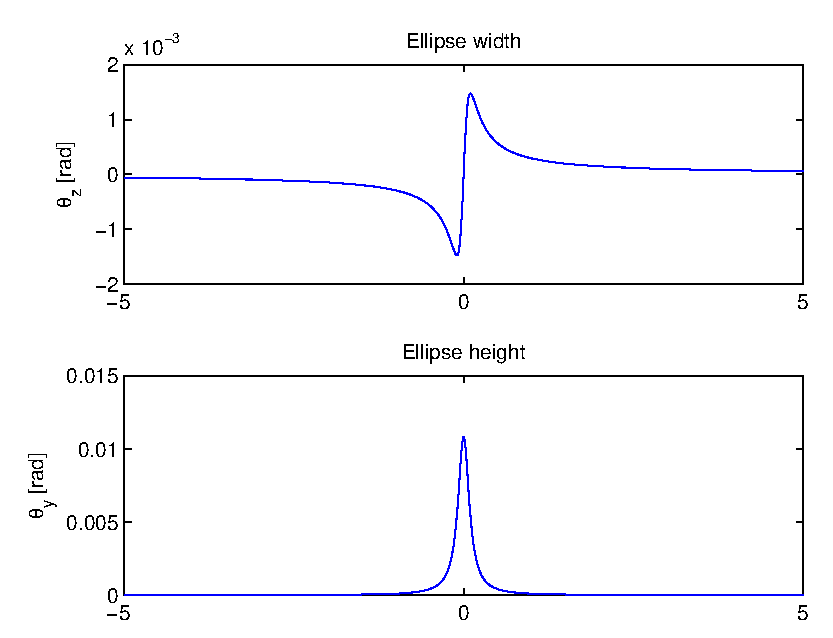
\includegraphics[width=0.9\linewidth]{figures/beam-deflection-script-02-elipse-width}
		\centering
		\caption{Το πλάτος και ύψος της έλλειψης στην αρχική κατάσταση}
		\label{fig:beam-deflection-script-02-elipse-width}
	\end{subfigure}
\caption{Απεικόνιση και στοιχεία της χαρακτηριστικής έλλειψης στην αρχική κατάσταση}
\label{fig:initial-ellipse}
\end{figure}

\begin{figure}[tph]	
	\begin{subfigure}{0.45\textwidth}
		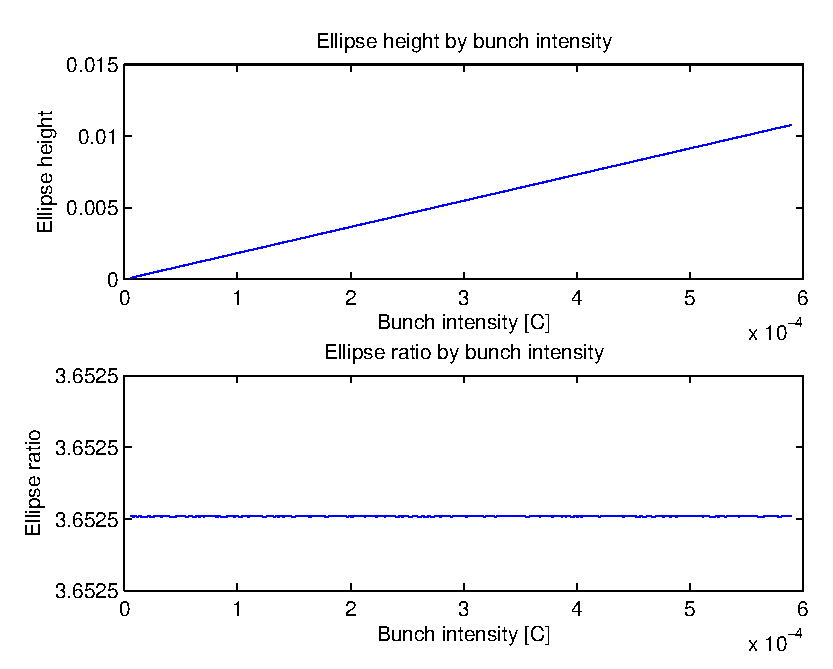
\includegraphics[width=0.9\linewidth]{figures/beam-deflection-script-03-elipse-height}
		\centering
		\caption{Επιρροή της έντασης της δέσμης ανίχνευσης στην ύψος και το λόγο της έλλειψης}
		\label{fig:beam-deflection-script-03-elipse-height}
	\end{subfigure}
	~
	\begin{subfigure}{0.45\textwidth}
		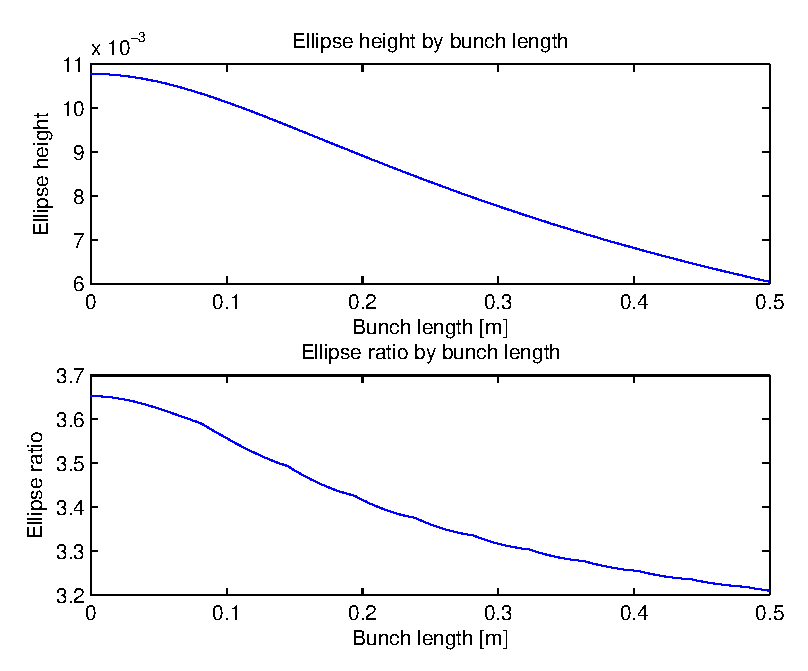
\includegraphics[width=0.9\linewidth]{figures/beam-deflection-script-04-elipse-height-by-bunch-intensity}
		\centering
		\caption{Επιρροή του μήκους της δέσμης ανίχνευσης στην ύψος και το λόγο της έλλειψης}
		\label{fig:beam-deflection-script-04-elipse-height-by-bunch-intensity}
	\end{subfigure}
	\par\bigskip
	\begin{subfigure}{0.45\textwidth}
		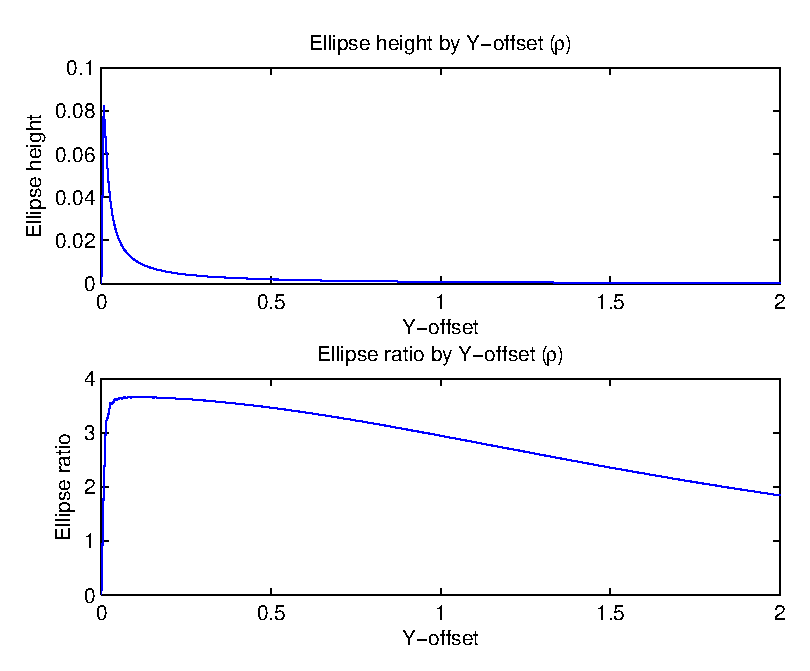
\includegraphics[width=0.9\linewidth]{figures/beam-deflection-script-05-elipse-ratio-by-bunch-intensity}
		\centering
		\caption[Επιρροή της αρχικής θέσης ριπής της δέσμης ανίχνευσης στην ύψος και το λόγο της έλλειψης]{Επιρροή της αρχικής θέσης ριπής ($Y$-\en{offset}) της δέσμης ανίχνευσης στην ύψος και το λόγο της έλλειψης}
		\label{fig:beam-deflection-script-05-elipse-ratio-by-bunch-intensity}
	\end{subfigure}
	~
	\begin{subfigure}{0.45\textwidth}
		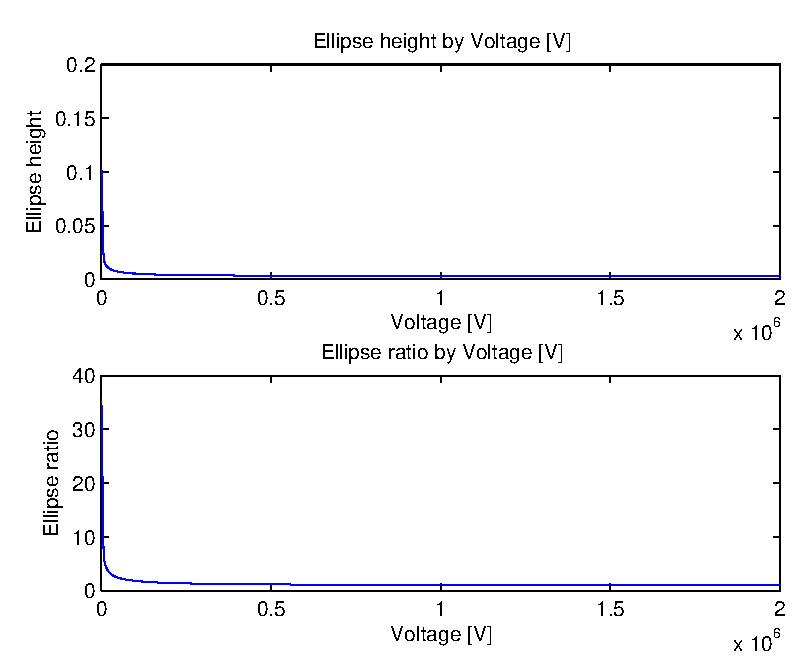
\includegraphics[width=0.9\linewidth]{figures/beam-deflection-script-06}
		\centering
		\caption{Επιρροή της γραμμικής μεταβολής τάσης της δέσμης ανίχνευσης στην ύψος και το λόγο της έλλειψης}
		\label{fig:beam-deflection-script-06}
	\end{subfigure}
	\par\bigskip
	\begin{subfigure}{0.45\textwidth}
		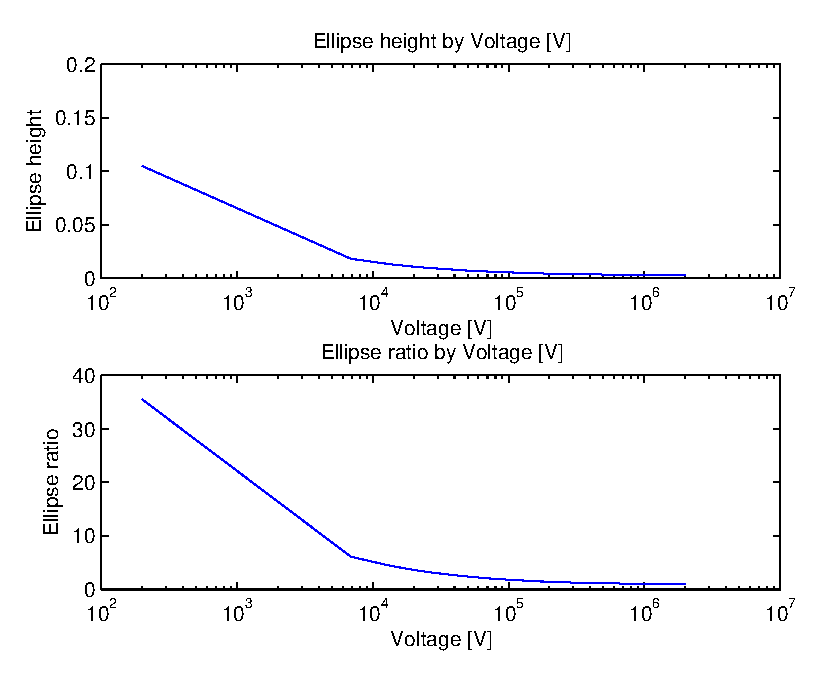
\includegraphics[width=0.9\linewidth]{figures/beam-deflection-script-07}
		\centering
		\caption{Επιρροή της εκθετικής μεταβολής τάσης της δέσμης ανίχνευσης στην ύψος και το λόγο της έλλειψης}
		\label{fig:beam-deflection-script-07}
	\end{subfigure}
\caption{Επιρροή διαφόρων μεγεθών στη χαρακτηριστική έλλειψη}
\label{fig:beam-deflectoin}
\end{figure}

\subsection{Αποτελέσματα προσομοίωσης}

\subsection{Σύγκριση αποτελεσμάτων}

\section{Αποτελέσματα προσομοίωσης της μεθόδου στο \en{CST}}


\section{Αποτελέσματα ανάλυσης με χρήση \en{CST} και \en{MATLAB}}




